\section{Object completion: selecting SA propagation}
\label{sec:sa}
\emph{Question: how should SA grow the core into the object?} A semantic core can be accurate yet incomplete. We therefore treat SA as a propagation operator, not as another class detector. One pass through all sixteen SA modules improves the frozen seed in the SA module screen, but the last 64-pixel module (\texttt{up\_blocks.3.attentions.2}, index 15) is better: OOF mIoU rises from 0.756 to 0.789 in the combined SA confirmation, and all five folds select this module. Its paired mean-image IoU gain is $+0.042$ with interval $[+0.037,+0.047]$. Eighteen classes improve; person loses 0.055, an early warning that diffusion can also erase or misassign object extent.

Separate screens favored call 30, resolutions 8+64 and heads $\{1,4,6\}$, but none survives the SA combination. With module 15 fixed, the head subset lowers mIoU by 0.002 and call 30 lowers it further. A Cartesian audit of six CA seeds and twelve SA settings plus no-SA controls retains the sequential CA/SA pair in all five folds. Module 15 is the best SA partner for every audited CA seed. This rules out the simple explanation that the sequential choice worked only because the CA seed happened to be frozen first.

\paragraph{How far should evidence propagate?}
With that same module, adding a second observation-wise pass raises OOF mIoU from 0.788 to 0.800 ($+0.012$); three passes are not promoted. The second pass particularly helps chair ($+0.078$) and person ($+0.030$). With the fixed DenseCRF added, the combined confirmation selects two passes plus R2 in all five folds and reaches 0.813 OOF, compared with 0.788 for one unrefined pass. Table~\ref{tab:stage_decisions} lists these same-study stages, without implying that the independent CA and SA screens are additive.

The mechanism is a completion--leakage tradeoff (Fig.~\ref{fig:propagation_depth}). In the diagnostic decomposition, pass two raises VOC recall from 0.912 to 0.924 at nearly unchanged precision; its largest mean image-IoU gain is in the lowest third of seed coverage ($+0.029$). A third pass adds pixels that are increasingly often wrong. A first-arrival diagnostic, recorded later with the SG25 package (A3 seed, calls 10--20, threshold 0.425), finds that pixels first accepted at depth one are 86.5\% true positive on VOC and 70.8\% on COCO, while pixels first accepted at depth three are only 39.3\% and 14.0\%. Further propagation therefore has diminishing reliability, especially under COCO clutter. These are diagnostic pixel statistics, not an alternative segmentation score.

\paragraph{Can a better graph replace plain propagation?}
If later arrivals cause the leakage, an operator that propagates more selectively should help. We registered and ran twenty-four families of alternatives against the one-pass reference (Fig.~\ref{fig:decision_map}a). Graph-restricting operators did not survive. An absorbing walk between confident foreground and background (SG1), confidence-locked propagation (SG3), reciprocal links (SG9), a seed-connected bottleneck (SG10), SA region labelling (SG4, SG13) and fourteen backlog operators, from DiffSeg-style merging to CA-weighted prototypes and seeded region growing, and none was promoted; several lost tens of points. The bottleneck score, for example, did not separate added true from false pixels (AUC 0.35--0.56).

One family did help: operators that weight or filter the 248 call--head observations by their agreement. Edge consensus (SG2), sign consensus (SG8), robust trimmed aggregation (SG11) and keeping the 50\% most consistent observations (SG12) each raised one-pass OOF mIoU from 0.787 to 0.797--0.798 and were promoted. This is, however, the level that a second pass already reaches (0.800). Applied on top of two passes, SG2 was retained by the plain two-pass reference in all five folds. Their per-class gains also resemble those of the second pass (class correlation 0.88 for SG2 and 0.82 for SG12; supplementary material). Observation reliability and a second pass are thus substitutes, two routes to object completion, not complementary gains. A separate temporal screen (SG18) promoted a middle-call window, calls 10--20, in all five folds.

\paragraph{Decision and next question.}
We freeze SA module 15, all calls and heads, and two observation-wise passes. The promoted alternatives were then carried to the full pipeline, which raised the next question: does a gain on the propagated map survive refinement?

\begin{figure*}[t]
\centering
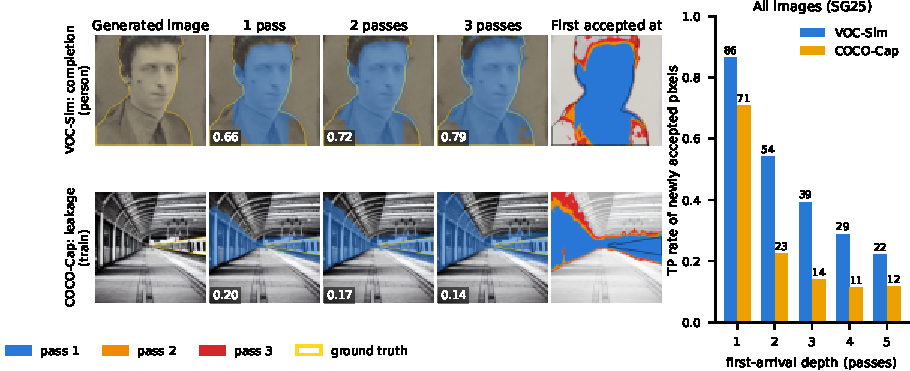
\includegraphics[width=\textwidth]{figures/propagation_depth.pdf}
\caption{\textbf{How far should evidence propagate?} Left: two images chosen by a fixed rule from the all-call raw maps of the SG22 run, without inspecting any image: on VOC-Sim, the image at the 90th percentile of the two-pass gain (completion); on COCO-Cap, the image at the 10th percentile of the three-pass gain (leakage). The supplementary material shows both rules on both datasets. Columns: the generated image with the ground-truth outline; the raw mask after one, two and three observation-wise passes at threshold 0.45, with the image IoU; and the pass at which each accepted pixel was first accepted. Right: the true-positive rate of newly accepted pixels at each depth, pooled over all 490 VOC-Sim and 707 COCO-Cap images, from the SG25 diagnostic (A3 seed, calls 10--20, threshold 0.425; depths 1--5). The third pass still helps the completion example, but pooled over images most pixels it first accepts are false positives on both datasets.}
\label{fig:propagation_depth}
\end{figure*}
